% A separate, self-contained five-page explanation of the completed project.
% Build: sh build_simple_report.sh
\documentclass[12pt,letterpaper]{article}
\usepackage[margin=0.82in,headheight=16pt]{geometry}
\usepackage[T1]{fontenc}
\usepackage[utf8]{inputenc}
\usepackage{helvet}
\renewcommand{\familydefault}{\sfdefault}
\usepackage{microtype,xcolor,fancyhdr,enumitem,tabularx,booktabs,array}
\usepackage{tikz}
\usetikzlibrary{arrows.meta,positioning}
\usepackage{hyperref}
\definecolor{ink}{HTML}{163640}
\definecolor{teal}{HTML}{117C77}
\definecolor{pale}{HTML}{EDF5F3}
\definecolor{muted}{HTML}{53666D}
\hypersetup{colorlinks=true,urlcolor=teal,linkcolor=teal,
  pdftitle={Manasi Project: A Simple Five-Page Guide},
  pdfauthor={Prepared for Manasi with Codex assistance},
  pdfsubject={A plain-language explanation of the parking-lot rainwater study}}
\setlength{\parindent}{0pt}
\setlength{\parskip}{8pt}
\setlength{\emergencystretch}{2em}
\setlength{\tabcolsep}{7pt}
\renewcommand{\arraystretch}{1.3}
\setlist{leftmargin=1.5em,itemsep=5pt,topsep=3pt}
\pagestyle{fancy}
\fancyhf{}
\fancyhead[L]{\small\color{ink}MANASI PROJECT \; / \; SIMPLE VERSION}
\fancyhead[R]{\small\color{muted}September 2026}
\fancyfoot[L]{\small\color{muted}A computer study of an imagined parking lot}
\fancyfoot[R]{\small\thepage\ of 5}
\renewcommand{\headrulewidth}{0.4pt}
\newcommand{\pagetitle}[2]{%
  {\small\bfseries\color{teal}#1\par}
  \vspace{3pt}{\LARGE\bfseries\color{ink}#2\par}\vspace{7pt}}
\newcommand{\smalltitle}[1]{\vspace{5pt}{\large\bfseries\color{ink}#1\par}}
\newcommand{\takeaway}[1]{\par\vspace{7pt}\noindent
  \colorbox{pale}{\parbox{\dimexpr\linewidth-2\fboxsep\relax}{%
    \vspace{5pt}\textbf{Main point:} #1\vspace{5pt}}}\par}
\newcolumntype{Y}{>{\raggedright\arraybackslash}X}
\begin{document}

\pagetitle{PAGE 1 \; / \; THE IDEA}{Slowing down rainwater}
\textbf{This project asks whether a holding area beside a parking lot can
stop too much rainwater from leaving the site all at once.}

When rain lands on a parking lot, some of it flows away. This moving
rainwater is called \textbf{runoff}. If lots of water arrives at a drain
at the same time, the drain may struggle to carry it away.

The idea is to collect that water in a shallow holding area and let it
leave through a small opening. Engineers call this \textbf{detention},
which simply means holding water for a while before releasing it.

\begin{center}
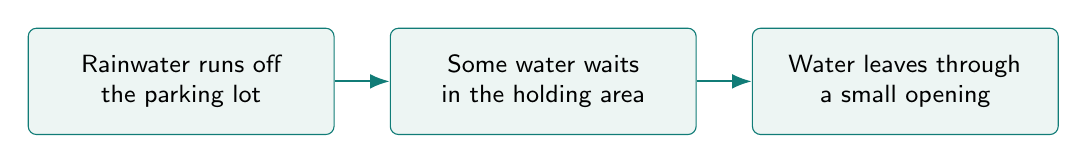
\begin{tikzpicture}[
  box/.style={draw=teal,fill=pale,rounded corners=3pt,align=center,
    text width=3.65cm,minimum height=1.35cm,font=\small},
  arrow/.style={-{Latex[length=2.5mm]},thick,teal},node distance=0.7cm]
\node[box] (lot) {Rainwater runs off\\the parking lot};
\node[box,right=of lot] (hold) {Some water waits\\in the holding area};
\node[box,right=of hold] (leave) {Water leaves through\\a small opening};
\draw[arrow] (lot)--(hold);
\draw[arrow] (hold)--(leave);
\end{tikzpicture}
\end{center}

\smalltitle{Think of a bathtub with the drain partly open}
If water enters faster than it leaves, the water level rises. After the
tap is turned off, the water keeps draining. The holding area works in a
similar way, but receives rainwater instead of water from a tap.

The opening matters. If it is too small, water may build up and spill out.
If it is too large, too much water may leave at once. The holding area also
needs enough room for the water that is waiting.

\smalltitle{The project had three goals}
\begin{enumerate}
\item Cut the amount of water leaving each second at the busiest moment
by at least half.
\item Keep water from spilling beyond the planned holding space.
\item Leave the holding area almost empty within 24 hours after the rain ends.
\end{enumerate}
The project looked for the smallest tested holding area that met all three
goals. It used an imagined site and computer calculations. No real basin
was built or tested. A \textbf{basin} is simply another name for the water
holding area.

\takeaway{The aim is to spread the water's release over time. The holding
area does not make the rainwater disappear.}

\newpage
\pagetitle{PAGE 2 \; / \; WHAT WAS TESTED}{One parking lot, many choices}
The imagined parking lot was 80 metres long and 50 metres wide. The holding
area beside it was 20 metres long and 10 metres wide. Its length and width
stayed the same. Its depth and opening changed between tests.

\smalltitle{Three amounts of rain}
Every test storm lasted one hour. The computer tried these rainfall amounts:
\begin{center}
\begin{tabularx}{0.94\linewidth}{YY}
\toprule
\textbf{Test} & \textbf{Rain falling in one hour} \\
\midrule
Smaller test & 2.5 centimetres \\
Main test used to choose a design & 5 centimetres \\
Larger test & 10 centimetres \\
\bottomrule
\end{tabularx}
\end{center}
\textbf{``5 centimetres of rain''} means the water would form a layer
5 centimetres deep if it all landed on a flat, waterproof surface and
none ran away.

\smalltitle{The timing of the rain also changed}
Each amount was tried three ways: \textbf{evenly spread},
\textbf{heavier at the start}, and \textbf{heavier at the end}.
This made nine rain tests. These were made-up storms, not local weather records.

\smalltitle{Different holding spaces and openings}
The study tried six holding sizes, from 30,000 to 180,000 litres. A litre
measures water amount: 30,000 litres would fill 30,000 one-litre bottles.
Square openings had sides of 4, 6, 8, or 10 centimetres.

Six holding sizes and four openings made \textbf{24 design choices}.
Trying each choice in all nine rain tests gave \textbf{216 computer tests}.

Every test counted rain on the lot \emph{and} the space beside it. Without
a holding area, rain from that extra space was assumed to run straight
away. With one, that water was held back too.

\takeaway{The chosen design had to pass all three timings of the main
5-centimetre rain test, not just the easiest one.}

\newpage
\pagetitle{PAGE 3 \; / \; HOW THE CHECKS WORKED}{Following the water, step by step}
The study used a \textbf{simulation}: a computer-based tryout of what might
happen. The computer followed the water through four simple steps.

\begin{enumerate}
\item \textbf{Work out how much rain reaches the holding area.}
The calculation assumed that a small amount of parking-lot rain would not
reach it. Rain landing directly on the holding area was also counted.

\item \textbf{Work out when the water arrives.}
Water does not arrive from every part of the parking lot at exactly the
same moment. The calculation allowed for that travel time.

\item \textbf{Keep track of water waiting and water leaving.}
At each small step in time, the computer added arriving water and
subtracted water leaving through the opening. If the holding space filled
up, extra water was counted as a spill. This is called \textbf{overflow}.

\item \textbf{Compare the choices.}
Each choice was compared with the same rain test without a holding area.
A choice passed only if it met all three project goals.
\end{enumerate}

\smalltitle{The busiest moment matters}
The report uses the term \textbf{peak flow}. This means the greatest amount
of water passing a point in one second during a test. It describes the
busiest moment, rather than the total water from the whole storm.

The project tried to make that busiest moment smaller. It also counted
spilled water as water leaving the site. Otherwise, an overflowing design
could look much better than it really was.

\smalltitle{How the calculations were checked}
The computer checked that all arriving water could be found again as water
that had left, spilled, or was still waiting. In this study, water in the
holding area was not allowed to soak into the ground or dry into the air.

There were \textbf{16 checks}, including no rain, a blocked opening, and
too little holding space. All passed. The study also repeated the tests
using smaller steps in time, ending at about two seconds per step. The
final two step sizes gave very similar answers and chose the same design.

\takeaway{These checks help show that the computer calculations work as
intended. They do not prove that an actual parking lot will behave exactly
the same way.}

\newpage
\pagetitle{PAGE 4 \; / \; THE RESULTS}{The smallest tested choice that passed}
\begin{center}
\colorbox{pale}{\parbox{0.91\linewidth}{\centering
\vspace{7pt}
{\Large\bfseries\color{ink}150,000 litres of holding space}\par
20 metres long, 10 metres wide, and 75 centimetres deep\par
\textbf{A square opening: 10 centimetres by 10 centimetres}
\vspace{7pt}}}
\end{center}
This choice passed all three main rain tests. No smaller tested holding
space passed all three. There might be a smaller choice between the sizes
that were tested; the study did not check every possible size.

\smalltitle{Much less water left at the busiest moment}
The table shows \textbf{litres per second}: how much water passed the
comparison point each second at the busiest moment of each test.
The numbers are rounded.

\begin{center}
\begin{tabularx}{\linewidth}{Yrr}
\toprule
\textbf{Rain timing} & \shortstack{\textbf{Without a}\\\textbf{holding area}} &
\shortstack{\textbf{With the}\\\textbf{chosen area}} \\
\midrule
Evenly spread & 57.5 & 21.2 \\
Heavier at the start & 73.2 & 21.0 \\
Heavier at the end & 85.7 & 21.9 \\
\bottomrule
\end{tabularx}
\end{center}
In every main test, the busiest flow was cut by \textbf{more than half}.
There was \textbf{no spill}, and the area became almost empty within
\textbf{about eight hours after the rain stopped}.

Here, ``almost empty'' means less than 1,500 litres remained. That is one
part out of every 100 parts the chosen area could hold. It does not mean
the area was completely dry. The deepest water in the main tests was about
69 centimetres, below the planned 75-centimetre limit.

\smalltitle{Why a smaller opening was not always better}
At the same 150,000-litre size, an 8-centimetre square opening released
water more slowly but caused a spill in one main test. Water arrived
faster than that smaller opening could let enough of it leave.

About 187,000 litres entered during each main test, even though the holding
space could only hold 150,000 litres at once. This worked because water
was already leaving while more water was arriving, just like a partly
draining bathtub.

\takeaway{The holding space and the opening need to work together. Slower
release helps only if there is enough room for the waiting water.}

\newpage
\pagetitle{PAGE 5 \; / \; WHAT IT MEANS}{A useful result, with clear limits}
\smalltitle{The larger rain tests were too much}
The chosen area worked in all the smaller 2.5-centimetre rain tests.
But in the 10-centimetre tests, it filled up and spilled about
\textbf{163,000 to 173,000 litres}. It barely reduced the busiest flow
in those larger tests. Having a holding area did not mean every rain test
was handled successfully.

\smalltitle{Changing a starting guess changed the answer}
An \textbf{assumption} is a starting idea used in a calculation when an
actual measurement is not available. This project made assumptions about
how much rain runs off the lot, how quickly it arrives, and how easily
water leaves through the opening.

The study changed these assumptions one at a time to see what happened.
When it assumed that \textbf{all} parking-lot rain became runoff, the
main test with heavier rain near the end caused a spill of about
2,800 litres. It also failed to cut the busiest flow by half.

So the chosen size worked with the original starting assumptions, but
\textbf{did not work under every condition that was tried}.

\smalltitle{What would be needed for a real site}
Someone would need to measure the actual ground, check local rainfall
information and rules for handling rainwater, and work out where water can safely go.
The shape and sides of the holding area, the real drain, and what happens
when the area fills up would also need proper design work.

The 75-centimetre depth in this study is a calculation limit, not a
finished instruction for building a pond. No real site was measured,
no basin was built, and no test at a real site was carried out.

\smalltitle{The lesson from the whole project}
The computer tests show that temporarily holding rainwater can greatly
reduce the busiest flow leaving a parking lot. They also show why the
holding space cannot be chosen by looking at only one storm or only the
size of the opening.

\takeaway{The smallest tested choice that worked for the main rain tests
held 150,000 litres and used a 10-centimetre square opening. It slowed
the water down, but it could still be overwhelmed.}

\vfill
{\small\color{muted}
\textbf{About this version.} This guide explains the saved results from
\texttt{manasi\_project}. The full engineering report contains the detailed
calculations and sources. Codex helped create the computer study and reports;
Manasi's own hands-on review is still to be recorded.}

\end{document}
